\section{数据分析记录}
考虑到未来职业发展, 无论哪行哪业, 数据可视化实用性强, 配置环境简单, 自学成本低, 是一个不错的突破口. 在网络上搜集了相关资料, python库很多, 还是从Panda开始学, 进行简单的可视化上手. 看了看官方教程, Panda库的核心在于数据类型Series和Frame. 

马上秋招开始了. 实现了简单的饼状图, 后续的日期分析还需要更深入的学习各种可视化库. 也不知道什么时候能抽时间做完:

\begin{itemize}
    \item 候选人备注的词云(可以用现成软件)
    \item 区域, 渠道来源的饼状图以及时间排序的堆积柱状图(可能Panda不支持), excel倒是很好实现.
\end{itemize}

\subsection{整体招聘数据分析}
在进行分析之前, 根据原始数据中的备注, 将候选人拒绝面试的原因一一归类, 整理为方便程序处理的格式, 这是一个纯手动的冗长过程. 整理过程认识到两点, 一是刚开始打电话时, 缺乏经验, 没有问候选人拒绝的具体原因; 另一方面, 记录比较繁琐, 难以整理. 这导致最后得出的结论一定是有失偏颇的. 不过本报告是为了记录AMS的生活和python可视化的结果, 至于最后的结论的正确与否, 是否可行, 不那么重要了.

如图~\ref{fig:0301}所示. 一共拨出电话450起, 其中371(90.5\%)起拒绝面试, 39(9.5\%)人愿意面试, 20(4.9\%)人真正到现场参加面试, 印象中大概4(1.0\%)人顺利入职, 一人为太仓客服, 孩子初中, 从朋友圈可看出小日子每天很幸福; 其他三人为叉车工, 其中一人是在上一章提到那位, boss上立马同意入职的电工. 其他两位是Miya交接. 

\begin{figure}[htbp]
    \centering
    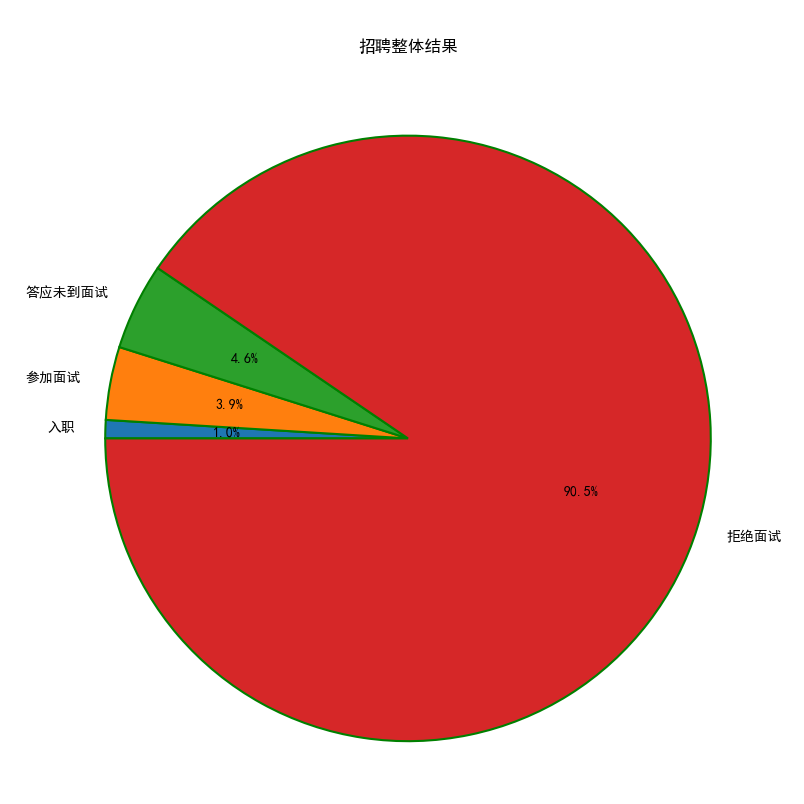
\includegraphics[height=18em]{pic/fig01_trim.png}
    \caption{招聘整体结果}
    \label{fig:0301}
\end{figure}

从招聘渠道看, 如图~\ref{fig:0302}所示, 前期主要使用51job中候选人的投递简历, 后期使用boss直聘直接寻找目标候选人, 因此两个网站比重较大(61\%). 其他招聘网站简历以辅助形式, 菁英网的候选人主要为区域性流动人口.

\begin{figure}[htbp]
    \centering
    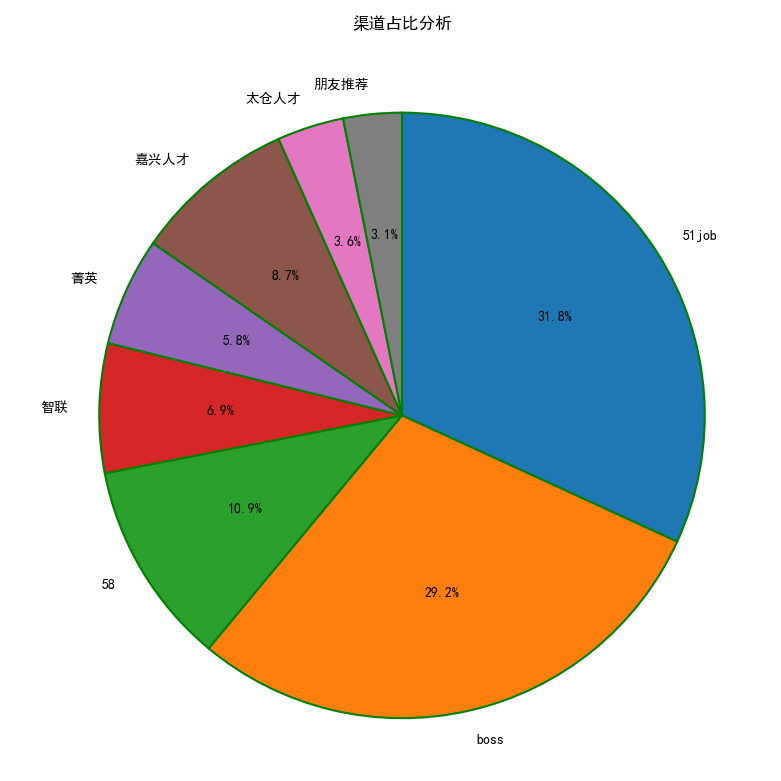
\includegraphics[height=18em]{pic/fig02_trim.png}
    \caption{渠道占比分析}
    \label{fig:0302}
\end{figure}

候选人拒绝职位的原因如图~\ref{fig:0303}所示. 原因有以下:
\begin{itemize}
    \item 无叉车证(8.8\%)
    \item 不做高叉(5.1\%)
    \item 不包吃住(12.6\%)
    \item 薪资过低(8.8\%)
    \item 距离过远(11.7\%)
    \item 拒绝夜班(5.3\%)
    \item 无法联系(27.5\%)
    \item 已找到工作(6.6\%)
    \item 疫情(1.3\%)
    \item 公积金(0.2\%)
    \item 无底薪且计件(1.5\%)
    \item 做六休一(0.2\%)
    \item 招聘网站信息错误或滞后(10.4\%)
\end{itemize}

\begin{figure}[htbp]
    \centering
    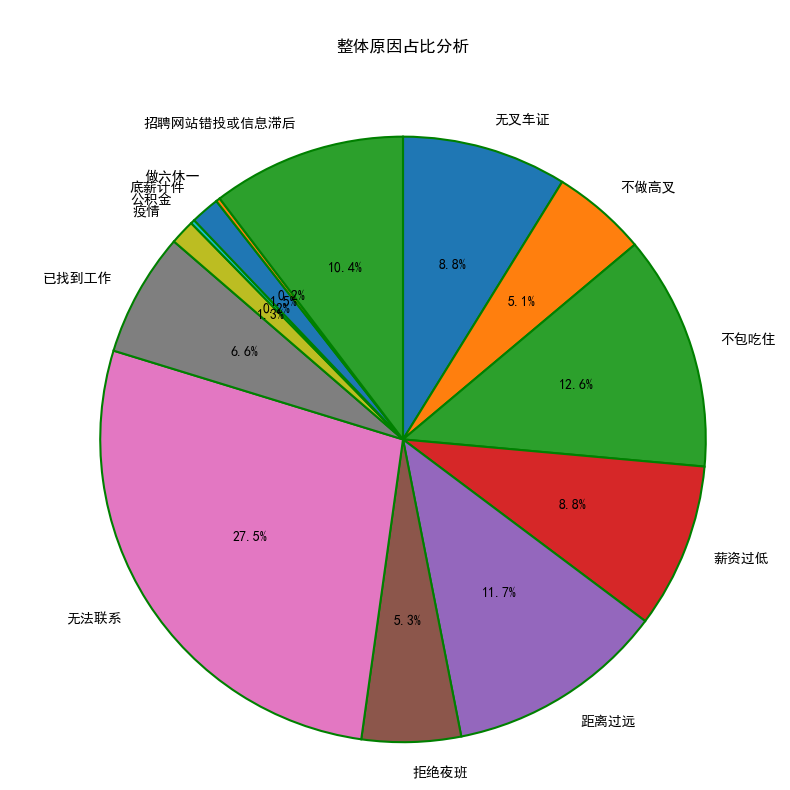
\includegraphics[height=18em]{pic/fig03_trim.png}
    \caption{整体原因分析}
    \label{fig:0303}
\end{figure}

``无叉车证''在上一章节提到过, 大部分国内物流公司招叉车工不需要叉车证, 有部分叉车工思维惯性认为JD只是说说而已, 抑或是存在侥幸心理. 其中``无法联系''的定义是, 当天三个电话皆未接, 次日继续三个电话依然未接, 则投入简历池, 等待下一位交接同事继续拨打电话. ``无法联系''占比最多, 个人认为由于蓝领受教育普遍程度较低, 不重视面试; 或是白天做工, 无法接电话, 导致只能在上班时间打电话的我无法与候选人取得联系, 并且我的电话是公号, 若不知分机号码, 叉车工师傅无法回我电话. 尽管我有两个手机号, 我认为公私分离是极为重要的. 

``不包吃住''和``距离过远''是有区别的. 后者的候选人已成家, 距离过远, 即便客户公司包吃住, 他们也不会来. 前者强调公司薪酬福利方面, 后者强调客户公司区位问题(远郊). 然而大部分由于``薪酬过低''拒绝面试的候选人在被询问原因时, 都会带上 ``不包吃住'', 两者强相关. 经验老道的叉车工师傅听到有底薪, 计件方式发钱, 往往也是拒绝, 印象中有许多候选人都因此拒绝, 但在图表中只有1.3\%, 大约5-6个人. 可惜的是, 今年七月份江苏疫情, 有个别愿意来客户公司工作的候选人因疫情原因拒绝了面试, 当然用疫情当借口另说. 另外, ``已找到工作'' 和 ``招聘网站错投或信息滞后'', 前者着重于候选人投递简历后很快找到工作, 其性质和后者截然不同, 后者为候选人完全没想换工作或是候选人根本没打算做叉车工但网站却神不知鬼不觉地帮候选人投递了客户公司相应岗位. 招聘网站刷数据般误投所体现出的无耻令人汗颜. 

总结整体招聘数据, 近四成拒绝率来自客户公司的薪资待遇, 工作时间, 绩效方式; 四成半是叉车工自身原因; 一成是招聘网站卖``假数据''; 剩下近一成为不可控因素. 

\subsection{各地招聘对比}

接下来对三个仓库的数据进行分析, 如图~\ref{fig:0304}. 

首先注意各个仓库的候选人联系数量, 嘉兴(242), 太仓(145), 上海(63). 联系数量主要和当地招聘难度和仓库招聘需求强相关. 嘉兴太仓很难招到合格候选人, 因此两地联系数量较多, 上海则不同. 

上海所有候选人都有叉车证. 虽统计样本较少, 即便如此, 预估上海候选人没有叉车证的概率也不会高于太仓候选人, 这并不能说明上海候选人素质更好, 只能说明嘉兴太仓两地候选人对规则的漠视, 即便看到JD上有硬性证件需求, 仍然发送简历, 契约精神更弱.  

另外, 上海候选人因薪资(18.2\%)和吃住(19.7\%)问题拒绝面试的原因远高于嘉兴(6.6\%, 10.3\%)和太仓(8.3\%, 12.4\%). 个人分析其背后原因, 一是城市. 上海经济发达, 相比四五线城市(县级市, 地级市)嘉兴太仓, 本身生活成本高; 二是区位. 上海仓库在上海交通大学附近, 附近房价四万至六万一平, 其周围房租两千至三千每人每月, 而嘉兴仓库和太仓仓库位于小城市的远郊, 附近房租则在三百至四百每人每月左右, 两者有近七八倍的差距. 这两点导致上海地域候选人对薪资和吃住问题极为看重. 

就电话面试质量来说, 上海候选人明显更健谈, 沟通效率更好, 也意味着他们社会经历丰富, 而嘉兴太仓无论从数据还是电话面试中的口音, 说话的连贯性和语气中体现的自信来讲, 都能感觉到, 虽同为叉车一行业, 却不是同一类叉车工. 上海候选人很快意识到客户公司的薪资极低, 迅速结束电话面试. 他们经常使用互联网, 经常登陆各个招聘网站或是软件, 因此招聘网站不会将其当作死用户自动替其投递简历, 图表中数据也证明了这一点, 上海由于招聘网站误投为3.0\%, 嘉兴为10.3\%, 太仓为13.8\%. 

\begin{figure}[!htbp]
    \centering
    \subfloat[嘉兴(242)招聘原因分析]{\label{fig:0304a}
    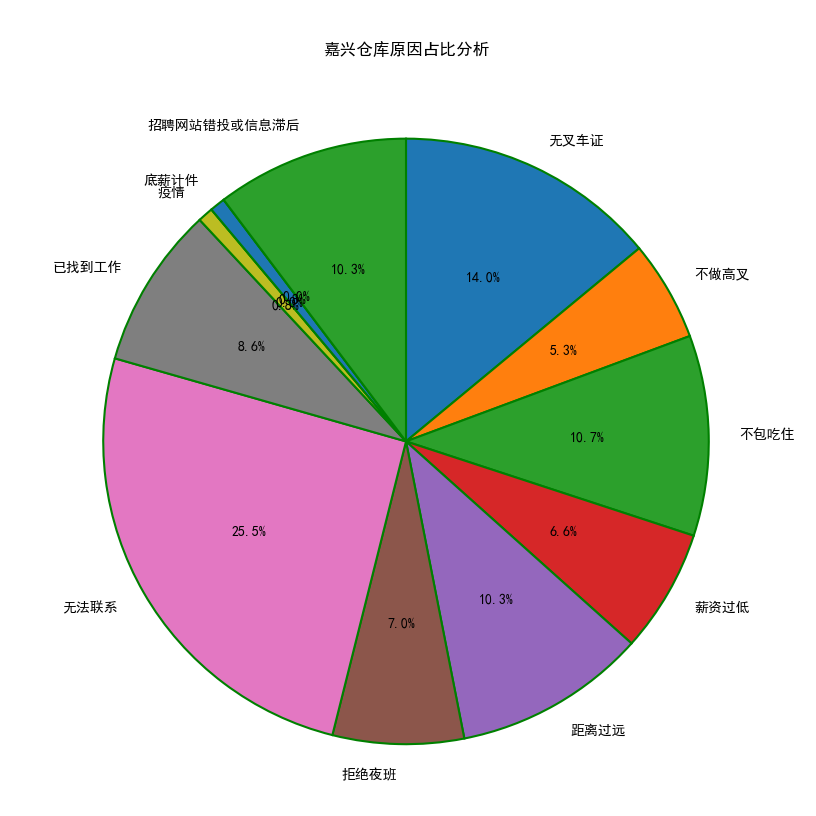
\includegraphics[height=15em]{pic/fig04_trim.png}}
    \qquad
    \subfloat[太仓(145)招聘原因分析]{\label{fig:0304b}
    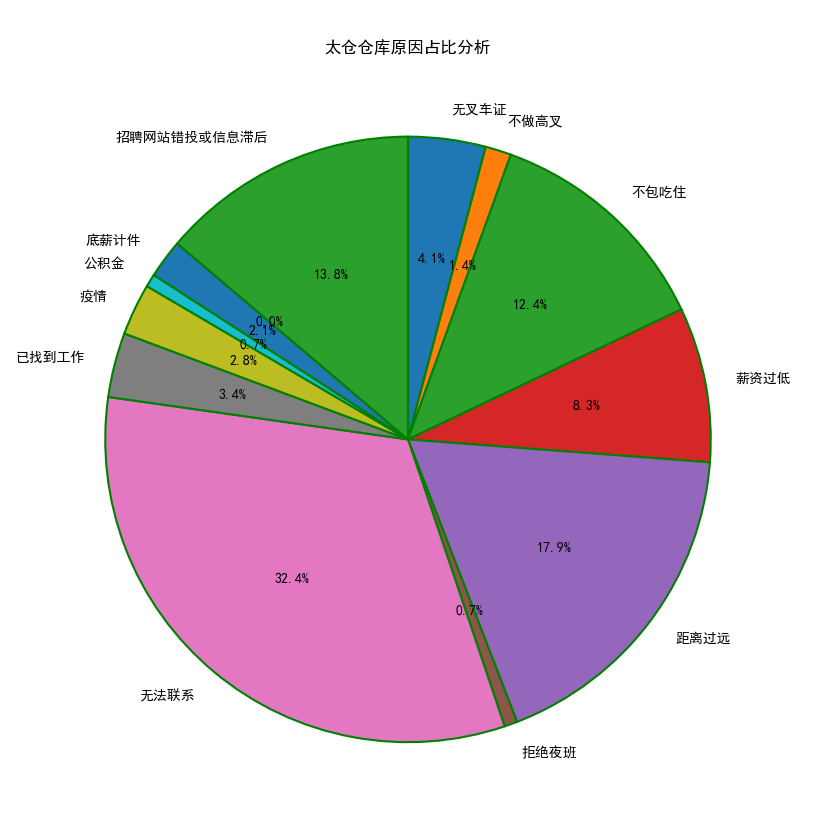
\includegraphics[height=15em]{pic/fig05_trim.png}}
    \\[12pt]
    \subfloat[上海(63)招聘原因分析]{\label{fig:0304c}
    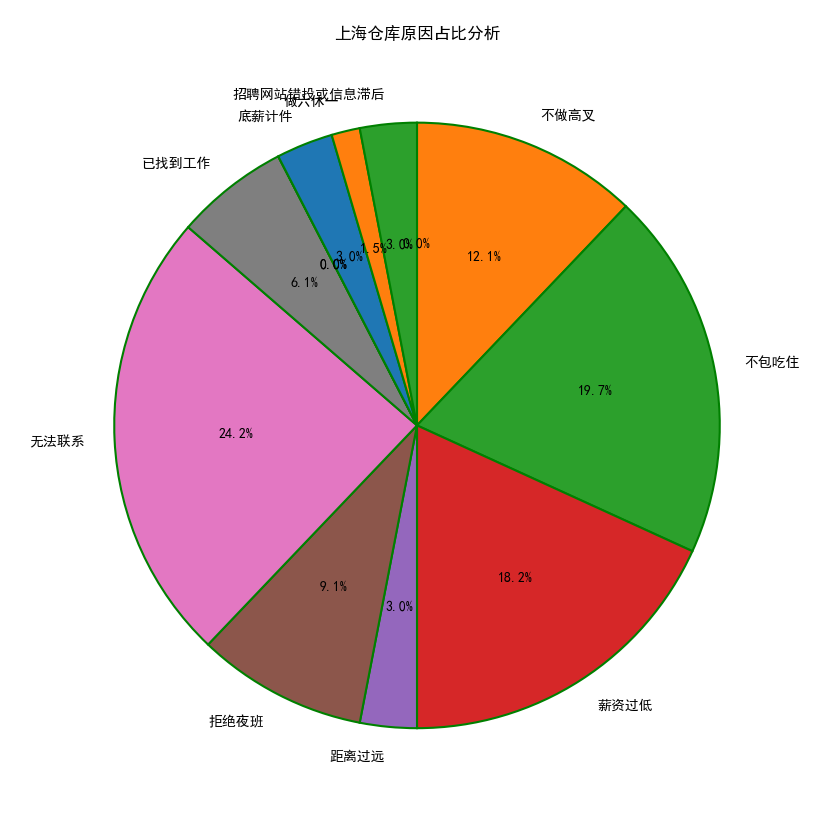
\includegraphics[height=15em]{pic/fig06_trim.png}}
    \caption{嘉兴太仓上海三地对比}
    \label{fig:0304}
\end{figure}

意外的是, 上海候选人(24.2\%)无法联系的比例(25.5\%)和嘉兴大致相同, 倒是太仓(32.4\%)独领风骚. 这一点虽可反驳我上一段看似充满地域性歧视的观点, 也可说明叉车行业候选人通病, 忙于工作不接电话. 也有可能是他们没法给我回电话, 哈哈. 拒绝夜班的比例, 太仓(0.7\%)远低嘉兴(7.0\%)上海(9.1\%)两地, 该现象的原因可能是大部分叉车工都已经因薪资和吃住问题拒绝了面试, 懒得提夜班? 

各种原因不做高位叉车的比例, 上海(12.1\%)远高于嘉兴(5.3\%)太仓(1.4\%)两地, 意味着上海叉车工的技能水平较嘉兴太仓低, 上海城市生活成本高, 吸引的更多是高科技人才, 相比之下, 有着低廉物价, 相对物价极高的工资的嘉兴和太仓更能吸引高质量叉车候选人, 然而这些高质量叉车工大几率是不会来客户公司.

然而数据还是不够多, 上海数据的说服力远不够.

但就我个人感受, 这一些数据居然已经把三地的叉车工简历池挖空, 快见底. 以上结论是否正确也有待考证. 

\subsection{简短的建议}
客户公司不可能给叉车工租房子, 涨工资或是改变绩效方式. 

AMS也不会为了一个没人愿意做的RPO项目, 就更改全公司的电话联系方式. 

我能做只有打多几通电话, 小小实习生而已.

\begin{flushright}
    \bfseries

    任家平

    二零二一年九月廿八日
\end{flushright}